\chapter[Chapter 2]{Solutions}

\subsection*{2-1}

It should be clear that the dot product of two vectors is independent of the reference frame used since the dot product can also be computed from $v_1 \cdot v_2 = |v_1| |v_2| \cos\theta$, i.e., it depends only on the magnitude of the two vectors and the angle between them.
\\~


Assume $v_1$, $v_2\space$ are vectors in $\R^3$. Introduce the notation $a=v_1$ and $b=v_2$.


Let $a^1$ and $b^1$ be the representation of the two vectors in frame $o_1x_1y_1z_1$ in $\R^3$.
Let $a^2$ and $b^2$ be the representation of the two vectors in a second frame $o_2x_2y_2z_2$ in $\R^3$, with the same origin as the first frame.

Let $R^1_2$ be the rotation matrix relating the two frames. Then we have 
\begin{align*} 
a^1 = R^1_2 a^2 \\ 
b^1 = R^1_2 b^2
\end{align*}

Writing the dot product equation we have, 
\begin{align*} 
a^1 \cdot b^1 &= (a^1)^T b^1 = (R^1_2 a^2)^T  R^1_2 b^2 = (a^2)^T (R^1_2)^T  R^1_2 b^2 \\
&= (a^2)^T b^2 = a^2 \cdot b^2 
\end{align*}
where we used the fact that $(R^1_2)^T  R^1_2 =I$

Hence, the dot product is independent from the choice of the reference frames.

\subsection*{2-2}

The length of a vector $v\in R^{n \times 1}$ is given by the 2-norm, $\|v\|_2 = \sqrt{v^Tv}$.\\~

Using the above, we have $\|Rv\|^2_2=v^TR^TRv=v^Tv=\|v\|_2^2$, where it was used that $R^TR=I$ for an orthogonal / rotation matrix.

\subsection*{2-3}

By denoting $d=p_1-p_2$, the relation becomes $\|d\|_2=\|Rd\|_2$, which is the same as the one in the exercise \textbf{2-2}

\subsection*{2-4}

Consider the 3D space. Let matrix $R\in \R^{3 \times 3}$ be represented by the column vectors
\begin{align*}
R = [ c_1 | c_2 | c_3 ]
\end{align*} 
where $c_i \space \in \R^{3 \times 1}, \space i=1,3$.
Then
\begin{align*}
R^T R = \left[\begin{array}{c} 
 c_1^T \\ 
 c_2^T \\ 
 c_3^T 
 \end{array} \right] \left[ c_1 | c_2 | c_3 \right] = \left[\begin{array}{ccc} 
 c_1^Tc_1 & c_1^Tc_2 & c_1^Tc_3 \\  
 c_2^Tc_1 & c_2^Tc_2 & c_2^Tc_3 \\ 
 c_3^Tc_1 & c_3^Tc_2 & c_3^Tc_3 \\ 
 \end{array}\right]
\end{align*}
In the case of an rotation matrix $R$, $R^TR=I$ implies 
\begin{align*}
 c_1^Tc_1 = 1, \quad c_1^Tc_2 = 0, \quad c_1^Tc_3 = 0 \\ 
  c_2^Tc_2 = 1, \quad c_2^Tc_1 = 0, \quad c_2^Tc_3 = 0 \\
   c_3^Tc_3 = 1, \quad c_3^Tc_1 = 0, \quad c_3^Tc_2 = 0
\end{align*}
which are exactly the relations that define the vectors $c_1$, $c_2$ and $c_3$ as being of unit length and mutually orthogonal. Note that the above derivation holds for any $R\in \R^{n\times n}$

\subsection*{2-5}
For any square matrix $A,B\in \R^{n \times n}$, the following hold:
\begin{align*}
&\det A = \det A^T \\
&\det(AB) = \det(A)\det(B)
\end{align*}
Therefore, for rotation matrices,  $R^T R = I $ implies
\begin{align*}
&\det R^TR= \det R^T \det R = (\det R)^2 = 1 \\
&\Rightarrow \det R = \pm 1
\end{align*} 

Let $R$ be given by
\begin{align*}
R &= [ c_1 | c_2 | c_3 ] \\
& = \left[\begin{array}{ccc} 
c_{11} & c_{12} & c_{13} \\  
c_{21} & c_{22} & c_{23} \\  
c_{31} & c_{32} & c_{33} \\   
\end{array}\right]
\end{align*}

Computing the determinant by selecting the last row gives
\begin{align*}
\det R &= c_{13} (c_{21}c_{32}-c_{22}c_{31}) \\
 & - c_{23} (c_{11}c_{32}-c_{12}c_{31}) \\
 & + c_{33} (c_{11}c_{22}-c_{21}c_{12}) \\
\end{align*}

As per definition, a right-handed coordinate frame defines the third coordinate axis to be given by $c_3 = c_1 \times c_2$. By definition of the cross-product, the components of $c_3$ along the $<i,j,k>$ unit vectors of the coordinate system are give by 
\begin{align}
&c_{13} = c_i := c_{21} c_{32} - c_{31} c_{22} \nonumber \\
&c_{23} = c_j := c_{31}c_{12} - c_{11}c_{32} \label{eq:cross_product_components} \\
&c_{33} = c_k := c_{11}c_{22} - c_{21}c_{12} \nonumber
\end{align} 

Using \eqref{eq:cross_product_components} in the expression of the determinant, one gets 
\begin{align*}
\det R &= c_{13}  c_{13} \\
& - c_{23} (-c_{23}) \\
& + c_{33} (c_{33}) \\
& = c_{13}^2 +c_{23}^2 + c_{33}^2  = +1
\end{align*}

\subsection*{2-6}

Straightforward to show
\begin{equation*}
R_{z,0} = I \quad (2.3)
\end{equation*} 
Simply replace $\theta = 0$ in equation \textbf{(2.2)} of the textbook.

To show
\begin{equation*}
R_{z,\theta} R_{z,\phi}= R_{z,\theta+\phi} \quad (2.4)
\end{equation*}
Perform the matrix multiplication to get
\begin{align*} 
R_{z,\theta} R_{z,\phi} &= \left[\begin{array}{ccc} 
(\cos\theta \cos \phi - \sin\theta \sin \phi) & (-\cos\theta \sin\phi - \sin\theta \cos\phi) & 0 \\  
(\sin\theta \cos\phi +\cos\theta \sin\phi) & (\cos\theta \cos \phi - \sin\theta \sin \phi) & 0 \\ 
0 & 0 & 1 \\   
\end{array}\right] \\
&=\left[\begin{array}{ccc} 
\cos(\theta + \phi)& -\sin(\theta + \phi) & 0 \\  
\sin(\theta + \phi) & \cos(\theta + \phi) & 0 \\ 
0 & 0 & 1 \\   
\end{array}\right] = R_{z,\theta+\phi}
\end{align*}

To show
\begin{equation*}
R_{z,\theta}^{-1} = R_{z,-\theta} \quad (2.5)
\end{equation*}
Either:
\begin{itemize}
	\item calculate the inverse of the matrix in equation \textbf{(2.2)} of the textbook and note that is exactly $R_{z,-\theta}$.
	\item use the fact that $R^{-1}=R^T$ for any rotation matrix and simply note that
	\begin{equation*}
	R_{z,\theta}^{-1} = R_{z,\theta}^{T} = R_{z,-\theta}
	\end{equation*}
	\item use (2.3) and (2.4) from the textbook to write
	\begin{align*}
	R_{z,\theta} R_{z,-\theta} &= R_{z,0} = I \\
	&\Rightarrow R_{z,-\theta} = R_{z,\theta}^{-1}
	\end{align*}
\end{itemize}

\subsection*{2-7}
$SO(n)$ is the group of orthogonal matrices for which 
\begin{align*}
R^T=R^{-1} \\
\det R=1
\end{align*}

\paragraph{Property 1:}  Let $A_1\in \R^{n\times n}$ and $A_2\in \R^{n\times n}$ be two orthogonal matrices for which the above to relations hold. Then, we have
\begin{align*}
(A_1*A_2)*(A_1*A_2)^T &= A_1*A_2 * A_2^T*A_1^T = A_1*A_2 * A_2^{-1}*A_1^{-1}= I
\end{align*}
Therefore 
\begin{align*}
(A_1*A_2)^T = (A_1*A_2)^{-1} 
\end{align*}
It is straightforward to show that $\det(A_1*A_2) = 1$.\\~\\
Hence $A_1*A_2 \in \space SO(n)$
\paragraph{Property 2:}  The relations holds in the more general case for the product of any three matrices $A_1\in \R^{n\times n}$, $A_2\in \R^{n\times n}$ and $A_3\in \R^{n\times n}$, not necessarily orthogonal.
\paragraph{Property 3:}  Let $A\in SO(n)$. TO show that there exists $\bar{A}\in SO(n)$ such that
\begin{align*}
A*\bar{A}_1 = \bar{A}_1*A = I 
\end{align*}
we simply note that $\bar{A}_1 = A^T$ satisfies the equation and that $A^T$ is also a matrix in $SO(n)$, while $I$ is the identity matrix of $\R^{n \times n}$.

\subsection*{2-8}
$\R_{x,\theta}$ represents the rotation about $x$ axis with angle $\theta$. Let the unit vectors for the initial and final rotated frame be denoted by $x_0,y_0,z_0$ and $x_1,y_1,z_1$ respectively, then by evaluating the direction cosines of the unit vectors, one gets:
\begin{align*}
	x_1 \cdot x_0 &= 1 \\
	x_1 \cdot y_0 &= 0 \\ 
	x_1 \cdot z_0 &= 0
\end{align*}
as the rotation is about the $x$ axis, and
\begin{align*}
y_1 \cdot x_0 &= 0 \\
y_1 \cdot y_0 &= \cos\theta \\
y_1 \cdot z_0 &= \cos(\frac{\pi}{2}-\theta) = \sin\theta
\end{align*}
\begin{align*}
z_1 \cdot x_0 &= 0 \\
z_1 \cdot y_0 &= \cos(\frac{\pi}{2}+\theta) = -\sin\theta \\
z_1 \cdot z_0 &=  \cos\theta; 
\end{align*}
which when put in matrix form results in the expression of equation \textbf{(2.6)}
\begin{align*}
\R_{x,\theta}=\left[\begin{array}{ccc} 
1 & 0 & 0 \\
0 & \cos\theta & -\sin\theta \\  
0 & \sin\theta &  \cos\theta    
\end{array}\right]
\end{align*}

Similarly to determine the expression of equation \textbf{(2.7)}, i.e., the case of a rotation about $y$ axis, the non-zero entries of the matrix are give by
\begin{align*}
x_1 \cdot x_0 &= \cos\theta \\
x_1 \cdot z_0 &= \cos(\frac{\pi}{2}+\theta) = -\sin\theta \\~\\
y_1 \cdot y_0 &= 1 \\~\\ 
z_1 \cdot x_0 &=  \cos(\frac{\pi}{2}-\theta) = \sin\theta \\
z_1 \cdot z_0 &=  \cos\theta; 
\end{align*}
which gives
\begin{align*}
\R_{y,\theta}=\left[\begin{array}{ccc} 
\cos\theta & 0 & \sin\theta \\
 0 & 1 & 0 \\  
-\sin\theta & 0 &  \cos\theta    
\end{array}\right]
\end{align*}

\subsection*{2-9}
Let 
\begin{align*}
A=\left[\begin{array}{cc} 
a & b \\
c & d 
\end{array}\right] \in \space SO(2)
\end{align*}
The inverse, $A^{-1}$ is given by
\begin{align*}
A^{-1}= \left[\begin{array}{cc} 
d & -b \\
-c & a 
\end{array}\right]
\end{align*}
Since $A^T=A^{-1}$ , then
\begin{align*}
\left[\begin{array}{cc} 
d & -b \\
-c & a 
\end{array}\right] =  \left[\begin{array}{cc} 
a & c \\
b & d 
\end{array}\right]
\end{align*}
then $d=a$ and $c=-b$. As a result $\det A = a^2 + b^2 = 1$. By selecting $\theta = \arctan (b/a)$, then we can choose $\cos\theta = a$ and $\sin\theta=b$, $\forall \theta \in [0,2\pi)]$.

\subsection*{2-10}

\begin{itemize}
	\item rotation about current frame: post-multiply
	\item rotation about fixed frame: pre-multiply
\end{itemize}

Solution: $R=R_{y,\psi}R_{x,\phi}R_{z,\theta}$

\subsection*{2-11}
\begin{itemize}
	\item rotation about current frame: post-multiply
	\item rotation about fixed frame: pre-multiply
\end{itemize}

Solution: $R=R_{z,\theta}R_{x,\phi}R_{x,\psi}$

\subsection*{2-12}
\begin{itemize}
	\item rotation about current frame: post-multiply
	\item rotation about fixed frame: pre-multiply
\end{itemize}

Solution: $R= R_{z,\alpha}R_{x,\phi}R_{z,\theta}R_{x,\psi}$

\subsection*{2-13}

\begin{itemize}
	\item rotation about current frame: post-multiply
	\item rotation about fixed frame: pre-multiply
\end{itemize}

Solution: $R= R_{z,\alpha}R_{z,\theta} R_{x,\phi}R_{x,\psi}$

\subsection*{2-14}
\begin{align*}
R &= R_{y,\frac{\pi}{2}} R_{x,\frac{\pi}{2}}=\\ 
&=\left[\begin{array}{ccc} 
0 & 0 & 1 \\
0 & 1 & 0 \\  
-1 & 0 & 0    
\end{array}\right]
\left[\begin{array}{ccc} 
1 & 0 & 0 \\
0 & 0 & -1 \\  
0 & 1 & 0    
\end{array}\right]\\
&=\left[\begin{array}{ccc} 
0 & 1 & 0 \\
0 & 0 & -1 \\  
-1 & 0 & 0    
\end{array}\right]
\end{align*}

Figure \ref{fig:ex2_14_sketch} shows a sketch of the rotations performed and the final frame orientation.
\begin{figure}[h]
	\caption{Transition from initial to final frame.}
	\centering
	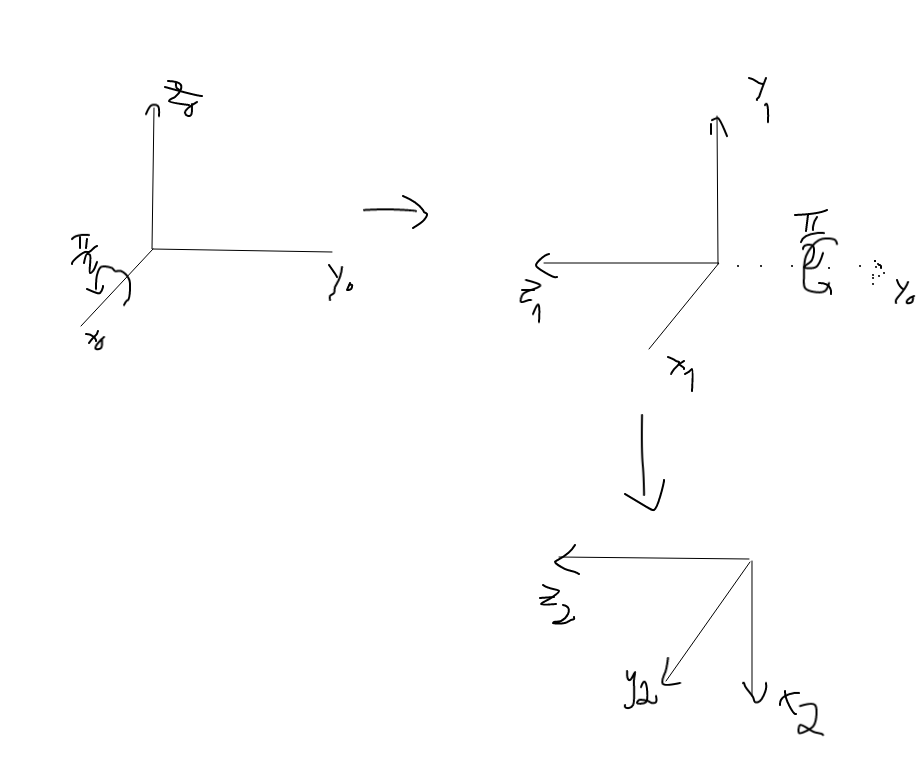
\includegraphics[scale=0.3]{./chapter02/figures/ex2_14.png}
	\label{fig:ex2_14_sketch}
\end{figure}

\subsection*{2-15}

\subsection*{2-16}

\subsection*{2-17}

\subsection*{2-18}

\subsection*{2-19}

\subsection*{2-20}